\documentclass[]{article}
\usepackage[spanish.mexico]{babel}
\usepackage[T1]{fontenc}
\usepackage[utf8]{inputenc}
%\usepackage{lmodern}
\usepackage[a4paper]{geometry}

\usepackage{amsmath}


%Graficos e imagenes
\usepackage{graphicx}
%\graphicspath{ Imagenes/ }

\usepackage{cite}

%Grafico de barras
%\usepackage{pgfplots}


\usepackage{tikz}
\usepackage[american voltages, american currents,siunitx]{circuitikz}

%\title{Proyecto de Optimización de Energía}
%\author{Pablo Vivar Colina}
%\date{Mayo 2018}



\begin{document}
	
%\usepackage[top=2cm,bottom=2cm,left=1cm,right=1cm]{geometry}


\begin{titlepage}
     \begin{center}
	
\includegraphics[width=0.09\textwidth]{UNAM}\Large Universidad Nacional Autónoma de México
        	
\includegraphics[width=0.09\textwidth]{FI}\\[1cm]
        \Large Facultad de Ingeniería\\[1cm]
       % \Large División de Ciencias Básicas\\[1cm]
         \Large Laboratorio de Fundamentos de Control(6655)\\[1cm]
         %la clave antes era:4314
         \footnotesize Profesor: Salcedo Ubilla María Leonor Ing.\\[1cm]
        \footnotesize Semestre 2019-1\\[1cm]
        
       

        \Large Práctica No. 1\\[1cm]
        
           

\Large Introdcción MATLAB
        
         %Texto a la derecha
          \begin{flushright}
\footnotesize  Grupo 2\\[0.5cm]
\footnotesize Brigada: 4\\[0.5cm]
\footnotesize Rodrigo Adrián Martínez López\\[0.5cm]
\footnotesize Vivar Colina Pablo\\[0.5cm]
 \end{flushright}
    %Texto a la izquierda
          \begin{flushleft}
        \footnotesize Ciudad Universitaria Agosto de 2018.\\
          \end{flushleft}
         
          
        %\vfill
        %\today
   \end{center}
\end{titlepage}
 %agregar portada
.\\[5cm]
%\maketitle

\tableofcontents  % Write out the Table of Contents

%\listoffigures  % Write out the List of Figures

\section{Versiones de telefonía celular}

\subsection{Generaciones de la Telefonía Celular}

En la sección anterior se presentó una muestra de la evolución de la telefonía
celular a lo largo de los años. Las distintas necesidades y avances dieron lugar a
generaciones tecnológicas bien diferenciadas que se comentan a continuación.\\

En dicha evolución se aprecia como se van cumpliendo las necesidades del
mercado para tener acceso múltiple al canal de comunicación, así como la
necesaria migración de los sistemas analógicos a sistema digital con el fin de
permitir mayor volumen de usuarios y ofrecer los niveles de seguridad que se
demandaban.\\

\subsection{Generación Cero (0G)}

0G representa a la telefonía móvil previa a la era celular. Estos teléfonos móviles
eran usualmente colocados en autos o camiones, aunque modelos en portafolios
también eran realizados. Por lo general, el transmisor (Transmisor-Receptor) era
montado en la parte trasera del vehículo y unido al resto del equipo (el dial y el
tubo) colocado cerca del asiento del conductor.
Eran vendidos a través de WCCs (Empresas Telefónicas alámbricas), RCCs
(Empresas Radio Telefónicas), y proveedores de servicios de radio doble vía.\\

 El
mercado estaba compuesto principalmente por constructores, celebridades, etc.
Esta tecnología, conocida como Autoradiopuhelin (ARP), fue lanzada en 1971 en
Finlandia; conocido ahora como el país con la primera red comercial de telefonía
móvil.\\

\subsection{Primera generación (1G)}

La 1G de la telefonía móvil hizo su aparición en 1979, si bien proliferó durante los
años 80. Introdujo los teléfonos “celulares”, basados en las redes celulares con
múltiples estaciones de base relativamente cercanas unas de otras, y protocolos
para el “traspaso” entre las celdas cuando el teléfono se movía de una celda a otra.\\

La transferencia analógica y estrictamente para voz son características
identificatorias de la generación. Con calidad de enlaces muy reducida, la
velocidad de conexión no era mayor a (2400 bauds). En cuanto a la transferencia
entre celdas, era muy imprecisa ya que contaban con una baja capacidad (Basadas
en FDMA, Frequency Division Multiple Access), lo que limitaba en forma notable
la cantidad de usuarios que el servicio podía ofrecer en forma simultánea ya que
los protocolos de asignación de canal estáticos padecen de ésta limitación.\\

Con respecto a la seguridad, las medidas preventivas no formaban parte de esta
primitiva telefonía celular. La tecnología predominante de esta generación es
AMPS (Advanced Mobile Phone System), desarrollada principalmente por Bell. Si
Telefonía celular
10bien fue introducida inicialmente en los Estados Unidos, fue usada en otros países
en forma extensiva. Otro sistema conocido como Sistema de Comunicación de
Acceso Total (TACS) fue introducido en el Reino Unido y muchos otros países.\\

Si bien había diferencias en la especificación de los sistemas, eran conceptualmente
muy similares. La información con la voz era transmitida en forma de frecuencia
modulada al proveedor del servicio. Un canal de control era usado en forma
simultánea para habilitar el traspaso a otro canal de comunicación de serlo
necesario. La frecuencia de los canales era distinta para cada sistema. MNT usaba
canales de 12.5KHz, AMPS de 30KHz y TACS de 25KHz.
A su vez, el tamaño de los aparatos era mayor al de hoy en día; fueron
originalmente diseñados para el uso en los automóviles. Motorola fue la primera
compañía en introducir un teléfono realmente portátil.
Motorola DynaTAC
Estos sistemas (NMT, AMPS, TACS, RTMI, C-Netz, y Radiocom 2000) fueron
conocidos luego como la Primera Generación (G1) de Teléfonos Celulares.\\

En Setiembre de 1981 la primera red de telefonía celular con roaming automático
comenzó en Arabia Saudita; siendo un sistema de la compañía NMT. Un mes más
tarde los países Nórdicos comenzaron una red NMT con roaming automático entre
países.\\

\subsection{Segunda generación (2G)}

Si bien el éxito de la 1G fue indiscutible, el uso masivo de la propia tecnología
mostró en forma clara las deficiencias que poseía. El espectro de frecuencia
utilizado era insuficiente para soportar la calidad de servicio que se requería. Al
convertirse a un sistema digital, ahorros significativos pudieron realizarse. Un
número de sistemas surgieron en la década del 90’ debido a estos hechos, y su
historia es tan exitosa como la de la generación anterior. La Segunda Generación
(2G) de telefonía celular, como ser GSM, IS-136 (TDMA), iDEN and IS-95 (CDMA)
comenzó a introducirse en el mercado.
La primera llamada digital entre teléfonos celulares fue realizada en Estados
Unidos en 1990. En 1991 la primera red GSM fue instalada en Europa.\\

Telefonía celular
11La generación se caracterizó por circuitos digitales de datos conmutados por
circuito y la introducción de la telefonía rápida y avanzada a las redes. Usó a su
vez acceso múltiple de tiempo dividido (TDMA) para permitir que hasta ocho
usuarios utilizaran los canales separados por 200MHz. Los sistemas básicos usaron
frecuencias de banda de 900MHz, mientras otros de 1800 y 1900MHz. Nuevas
bandas de 850MHz fueron agregadas en forma posterior. El rango de frecuencia
utilizado por los sistemas 2G coincidió con algunas de las bandas utilizadas por los
sistemas 1G (como a 900Hz en Europa), desplazándolos rápidamente.\\

La introducción de esta generación trajo la desaparición de los “ladrillos” que se
conocían como teléfonos celulares, dando paso a pequeñísimos aparatos que
entran en la palma de la mano y oscilan entre los 80-200gr. Mejoras en la duración
de la batería, tecnologías de bajo consumo energético.
Teléfono GSM de diseño regular
EL sistema 2G utiliza protocolos de codificación más sofisticados y se emplea en
los sistemas de telefonía celular actuales. Las tecnologías predominantes son: GSM
(Global System por Mobile Communications); IS-136 (conocido también como
TIA/EIA136 o ANSI-136) y CDMA (Code Division Multiple Access) y PDC
(Personal Digital Communications), éste último utilizado en Japón. Se encontrará
información detallada de los protocolos en la sección correspondiente más
adelante.\\

Los protocolos empleados en los sistemas 2G soportan velocidades de información
por voz más altas, pero limitados en comunicación de datos. Se pueden ofrecer
servicios auxiliares, como datos, fax y SMS (Short Message Service). La mayoría de
los protocolos de 2G ofrecen diferentes niveles de encripción. En Estados Unidos y
otros países se le conoce a 2G como PCS (Personal Communication Services).\\

\subsection{Generación 2.5 G}

Una vez que la segunda generación se estableció, las limitantes de algunos
sistemas en lo referente al envío de información se hicieron evidentes. Muchas
aplicaciones para transferencia de información eran vistas a medida que el uso de
laptops y del propio Internet se fueron popularizando. Si bien la tercera generación
estaba en el horizonte, algunos servicios se hicieron necesarios previa a su llegada.
El General Packet Radio Service (GPRS) desarrollado para el sistema GSM fue de
los primeros en ser visto. Hasta este momento, todos los circuitos eran dedicados
en forma exclusiva a cada usuario. Este enfoque es conocido como “Circuit
Switched”, donde por ejemplo un circuito es establecido para cada usuario del sistema.\\

Telefonía celular

Esto era ineficiente cuando un canal transfería información sólo en un
pequeño porcentaje. El nuevo sistema permitía a los usuarios compartir un mismo
canal, dirigiendo los paquetes de información desde el emisor al receptor. Esto
permite el uso más eficiente de los canales de comunicación, lo que habilita a las
compañías proveedoras de servicios a cobrar menos por ellos.\\

Aún más cantidad de mejoras fueron realizadas a la taza de transferencia de
información al introducirse el sistema conocido como EDGE (Enhanced Data rates
aplicado a GSM Evolution). Éste básicamente es el sistema GPRS con un nuevo
esquema de modulación de frecuencia.
Mientras GPRS y EDGE se aplicaron a GSM, otras mejoras fueron orientadas al
sistema CDMA, siendo el primer paso de CDMA a CDMA2000 1x.\\

2.5G provee algunos de los beneficios de 3G (por ejemplo conmutación de datos en
paquetes) y puede usar algo de la infraestructura utilizada por 2G en las redes
GSM and CDMA. La tecnología más comunmente conocida de 2.5G es GPRS
(nombrada anteriormente), que provee transferencia de datos a velocidad
moderada usando canales TDMA no utilizados en la red GSM. Algunos
protocolos, como ser EDGE para GSM y CDMA2000 1x-RTT para CDMA, califican
oficialmente como servicios "3G" (debido a que su taza de transferencia de datos
supera los 144 kbit/s), pero son considerados por la mayoría como servicios 2.5G
(o 2.75G, que luce aún mas sofisticado) porque son en realidad varias veces más
lentos que los servicios implementados en una red 3G.
Mientras los términos "2G" y "3G" están definidos oficialmente, no lo está "2.5G".
Fue inventado con fines únicamente publicitarios.
Muchos de los proveedores de servicios de telecomunicaciones se moverán a las
redes 2.5G antes de entrar masivamente a la 3. La tecnología 2.5G es más rápida, y
más económica para actualizar a 3G.\\

\subsection{Tercera generación (3G).}

No mucho luego de haberse introducido las redes 2G se comenzó a desarrollar los
sistemas 3G. Como suele ser inevitable, hay variados estándares con distintos
competidores que intentan que su tecnología sea la predominante. Sin embargo, en
forma muy diferencial a los sistemas 2G, el significado de 3G fue estandarizado
por el proceso IMT-2000. Este proceso no estandarizó una tecnología sino una serie
de requerimientos (2 Mbit/s de máxima taza de transferencia en ambientes
cerrados, y 384 kbit/s en ambientes abiertos, por ejemplo). Hoy en día, la idea de
un único estándar internacional se ha visto dividida en múltiples estándares bien
diferenciados entre sí.\\

Existen principalmente tres tecnologías 3G. Para Europa existe UMTS (Universal
Mobile Telecommunication System) usando CDMA de banda ancha (W-CDMA).
Este sistema provee transferencia de información de hasta 2Mbps.
Telefonía celular
13Están a su vez las evoluciones de CDMA2000. La primera en ser lanzada fue
CDMA2000 1xEV-DO, donde EV-DO viene de Evolution Data Only. La idea atrás
de este sistema era que muchas de las aplicaciones sólo requirieran conexión de
datos, como sería el caso si se usara el celular para conectar una PC a Internet en
forma inalámbrica. En caso de requerir además comunicación por voz, un canal 1X
estándar es requerido. Además de usar tecnología CDMA, EV-DO usa tecnología
TDMA para proveer de la velocidad de transferencia necesaria y mantener la
compatibilidad con CDMA y CDMA2000 1X.
La siguiente evolución de CDMA2000 fue CDMA2000 1xEV-DV. Esto fue una
evolución del sistema 1X totalmente distinto a CDMA2000 1xEV-DO, ofreciendo
servicios totales de voz y datos. Este sistema también es compatible con CDMA y
CDMA2000 1X y es capaz de ofrecer tasas de transferencia de 3.1Mbps.
Estos dos protocolos usaron lo que se conoce como FDD (Frequency Division
Duplex), donde los links de ida y vuelta usan distintas frecuencias. Dentro de
UMTS existe una especificación conocida como TDD (Time Division Duplex),
donde los links poseen la misma frecuencia pero usan distintos segmentos de
tiempo. Sin embargo, TDD no se implementará en los mercados por un tiempo.
Un tercer sistema 3G fue desarrollado en China que usa TDD. Conocido como TD-
SCDMA (Time Division Synchronous CDMA), usa un canal de 1.6MHz y fue
pensado para que abarque el mercado Chino y de los países vecinos.\\

Algunos de los sistemas 2.5G, como ser CDMA2000 1x y GPRS, proveen de
algunas de las funcionalidades de 3G sin llegar a los niveles de transferencia de
datos o usos multimedia de la nueva generación. Por ejemplo, CDMA2000-1X
puede, en teoría, transferir información hasta a 307 kbit/s. Justo por encima de esto
se encuentra el sistema EDGE, el cual puede en teoría superar los requerimientos
de los sistemas 3G; aunque esto es por tan poco que cualquier implementación
práctica quedaría probablemente por debajo del límite deseado.
Al comienzo del siglo 21, sistemas 3G como UMTS y CDMA2000 1xEV-DO han
comenzado a estar al alcance del público en los países del primer mundo. Sin
embargo, el éxito de estos sistemas aún está por probarse.\\

\section{Tendencias en telefonía celular, como se emplea y como se espera emplearse}

Para los consumidores, la tecnología 5G no implica solo un
Internet móvil más rápido, sino, sobre todo, una conectividad
a Internet en muchos más objetos que los que se ven hoy en
día, en 2016. Los vehículos y los hogares son dos ejemplos de
la gran revolución del IoT que se avecina, con el apoyo de las
redes 5G.\\

\begin{figure}[h!]
	\centering
	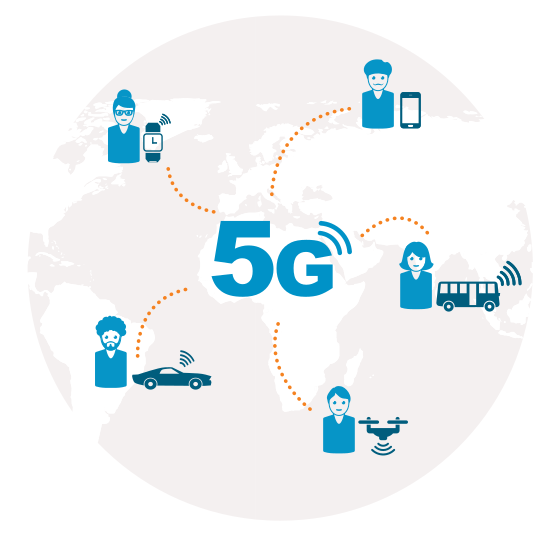
\includegraphics[width=0.6\textwidth]{Imagenes/5Gapp.png}
	\caption{Networking 5G}
	\label{fig:5Gapp}
\end{figure}

La tecnología inalámbrica Wi-Fi es una tecnología de "red de
área local", limitada en el alcance de su funcionamiento y muy
limitada en velocidad, así como en latencia. Muchos de los
servicios del IoT están exigiendo mayor ubicuidad, mayor
movilidad, mayor rendimiento en cuanto a la velocidad, y mayor
respuesta en cuanto al tiempo. Realmente la tecnología 5G va a
desatar un verdadero ecosistema del IoT.\\


\section{¿Como incidirá 5G en las áreas de trabajo?}


Algunas aplicaciones clave, como los vehículos autónomos,
requieren una latencia muy agresiva (tiempo de respuesta
rápido), si bien no requieren altas tasas de datos.
Por el contrario, los servicios empresariales basados en la
nube con análisis masivo de datos van a requerir mejoras de
velocidad más que de latencia.\\

\begin{figure}[h!]
	\centering
	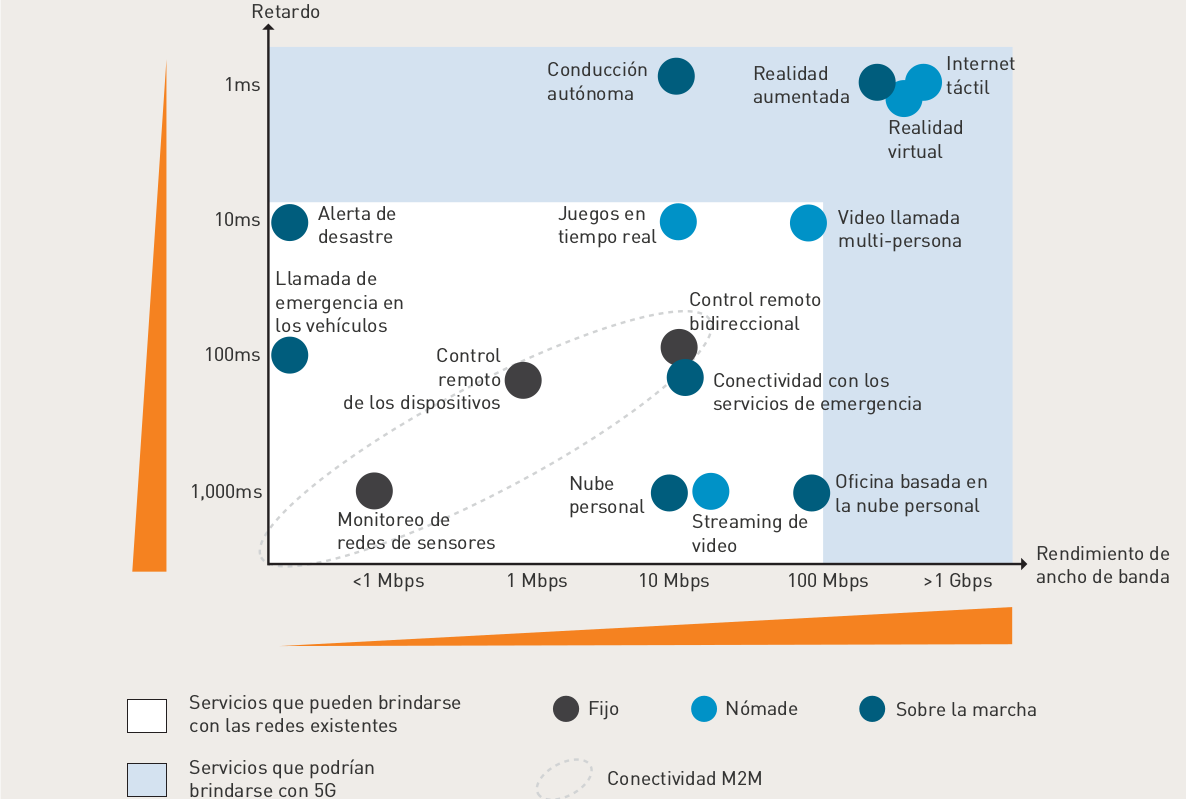
\includegraphics[width=0.6\textwidth]{Imagenes/sist1.png}
	\caption{Rendimiento de ancho de banda contra retardo}
	\label{fig:sist1}
\end{figure}


En la figura \ref{fig:sist1} podemos apreciar como la productividad en áreas de trabajo y otras puede ser afectada por el ancho de banda en las telecomunicaciones de manera positiva.\\


\section{¿Será posible la videoconferencia por medios móviles?}


\subsection{Internet táctil}

Definido como aplicaciones de
Internet de súper baja latencia
para cumplir el tiempo de
respuesta de nivel humano. Por
ejemplo, para la nanocirugía, los
sistemas de robótica
intracorporales van a permitir que
los cirujanos lleven a cabo el
micro mecanizado en tiempo real.
El impacto del Internet táctil
también va a revolucionar la
industria del juego.\\

\begin{figure}[h!]
	\centering
	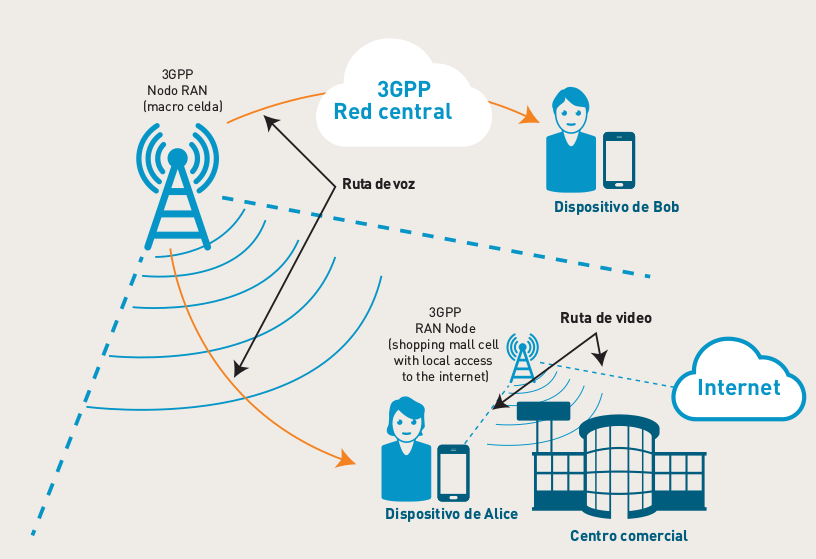
\includegraphics[width=0.6\textwidth]{Imagenes/sist2.png}
	\caption{Diagrama de telecomunicaciones de dispositivos móviles}
	\label{fig:sist2}
\end{figure}

 También se va
a extender a los otros cuatro
sentidos humanos más allá del
tacto (el oído, la vista, el olfato, el
gusto), para permitir nuevas
interfaces de usuario de realidad
virtual donde las aplicaciones van
a cumplir el tiempo de respuesta
de los sentidos humanos.\\

En la figura \ref{fig:sist2} podemos apreciar la interacción dinámica de los dispositivos móviles con los medios de telecomunicaciones.\\

\section{¿El avance en la tecnología incidirá con Voz sobre el internet, el internet de las cosas?}


\subsection{Qué es el Internet de las Cosas}

Una expresión extraña que provoca dudas y perplejidad en las cabezas de más de uno. El Internet de las Cosas, abreviado como IoT, es un neologismo que fue utilizado por primera vez en 1999 por Kevin Ashton, cofundador y director de Auto-ID Center, para referirse a todos aquellos dispositivos (aparte del ordenador y el smartphone) conectados a internet. Ya se trate de vehículos, sensores de fitness, frigoríficos, bombillas o elementos de mobiliario, todos están conectados a Internet y pueden recoger e intercambiar datos a través del uso de sensores.\\

Respondiendo la pregunta:\\

Sí, cualquier objeto conectado a Internet y monitorizable de forma remota puede formar parte de este mundo mágico, pero para entender cómo nos afectará el Internet de las Cosas puede ayudar aclarar en qué ámbitos- en constante aumento- se utilizará.\\

\subsection{En el hogar}

Los asistentes digitales comienzan a llamar a la puerta para hacer de nuestros hogares “hogares inteligentes”. El IoT controlará nuestros hogares a distancia, vigilará a los niños mientras duermen en la habitación de al lado, apagará el horno tan pronto como el bizcocho esté listo, ajustará las luces en la sala de estar dependiendo de nuestras necesidades, eso  y mucho más con sencillas órdenes de voz.\\

\subsection{En la ciudad}

Barcelona, sede del MWC, es el mejor ejemplo de Smart City que podemos plantear en este momento. Desde 2012, la capital catalana ha comenzado a utilizar el IoT para la gestión del transporte (paradas de bus digitales, coches eléctricos, bicicletas públicas, gestión de aparcamientos, a través de sensores colocados en el asfalto, etc.), la iluminación de la ciudad (lámparas LED que sirven también como puntos WiFi) y la gestión de los espacios verdes (el IoT permite controlar los aspersores). Todo esto ha sido posible gracias a la red y la extensión de cables de fibra óptica en la ciudad.\\

\subsection{En el coche}

Gracias a los sensores integrados, los semáforos se ponen en verde en cuanto el camino está despejado.  Y esto es sólo un ejemplo de los campos de aplicación del IoT si hablamos de coches y de conducción. Los coches serán más independientes y capaces de garantizar una mayor seguridad utilizando los sensores, la disponibilidad constante de datos y el potencial del 5G.\\

\subsection{En el gimnasio o al aire libre}

Los SmartBand son probablemente los dispositivos IoT más conocidos en la actualidad y permiten supervisar la actividad física y el sueño. Las nuevas generaciones son cada vez más inteligentes y permiten recoger más y más datos con el fin de ofrecer un mejor rendimiento tanto en el gimnasio como al aire libre, tomando en cuenta las condiciones meteorológicas, el estado físico, las variables ambientales. Y de simples puntos de referencia para la actividad física, pasarán a ser cada vez más útiles para el seguimiento de nuestra salud y para comunicarse con los especialistas y centros médicos. Google, sólo por poner un ejemplo, está trabajando desde hace tiempo en unas lentillas capaces de medir la glucosa para hacer la vida más fácil de los diabéticos.\\

\subsection{Conclusión}

El Internet de las Cosas va a cambiar, o más bien está empezando a cambiar el mundo del trabajo y nuestro día a día. No será un camino de rosas. Con el IoT vamos a hacer frente a varios desafíos, en primer lugar el de la seguridad. Proteger la avalancha de datos necesarios para permitir la comunicación de estos dispositivos no será fácil, serán necesarias nuevas reglas para proteger la privacidad, pero sobre esto ya hablaremos más adelante en otro artículo.\\

 
%AQUI VAMOS

\section{¿Qué técnicas de modulación se emplearán en 5G?}

\subsection{Nuevas formas de onda}

Una forma de onda ideal para los sistemas 5G deberá ser lo suficientemente flexible para soportar varios escenarios con diferentes tipos de tráfico, como son los móviles de banda ancha aumentada eMBB (enhanced Mobile BroandBand), las comunicaciones masivas entre dispositivos mMTC (massive Machine Type Communications) y comunicaciones muy fiables de baja latencia URLLC (Ultra Reliable Low Latency Communications) en diferentes entornos (rural, urbano, interiores) y una amplia gama de velocidades de desplazamiento. Por todo ello debería cumplir los siguientes requisitos:

\begin{itemize}
	\item Las subportadoras deberán ser mutuamente ortogonales en tiempo y frecuencia para que la interferencia interportadoras (ICI) sea lo más reducida posible. 
	\item Las señales deben estar bien localizadas en el tiempo y frecuencia, para que la interferencia entre símbolos (ISI) debida a la dispersión temporal y la ICI originada por la dispersión Doppler sean prácticamente nulas. Además una buena localización temporal es necesaria para tener una latencia reducida. 
	\item Máxima eficiencia espectral (bits/s/Hz)
	No obstante, es bien conocido por la teoría de la señal que no es posible satisfacer estos requisitos simultáneamente, por lo que habrá que aceptar soluciones de compromiso que potencien alguna característica a costa de las otras. Por ello, se propone aligerar las exigencias de ortogonalidad y estricta sincronización que rigen en 4G/LTE empleando nuevas señales no ortogonales. 
\end{itemize}

Esto conlleva admitir cierta interferencia entre subportadoras y entre símbolos, pero controlando sus efectos mediante técnicas adecuadas de filtrado en transmisión y recepción con el uso de los llamados filtros prototipo PF (Prototype Filters) configurables.
Siguiendo estas pautas, las formas de onda derivadas de OFDM que se están estudiando como candidatas para 5G y que utilizan filtros prototipo, pueden clasificarse por el tipo de procesado de convolución (circular para el caso de señales que se repiten periódicamente, lineal para el contrario):

\begin{itemize}
	\item Convolución lineal: Filter Bank MultiCarrier (FBMC), Universal Filtered MultiCarrier (UFMC).
	\item Convolución circular: Generalized Frequency Division Multiplexing (GFDM), Circular filter bank multicarrier (C-FBMC). 
	
\end{itemize}

Seguidamente se presenta una visión general de las tres primeras.

\subsection{Generalized Frequency Division Multiplex (GFDM) 
	}
	
Una de las soluciones que aparecen de forma natural al intentar solucionar el problema de la interferencia entre portadoras es la de utilizar un filtro para cada una de ellas, que evite el desbordamiento de la señal de cada subportadora hacia las demás. Es lo que se hace por ejemplo en la opción $GFDM$, que es un sistema de modulación multiportadora no ortogonal con filtrado individual de cada subportadora, mediante un filtro prototipo configurable individualmente. Los datos a transmitir son símbolos de modulación complejos procedentes de una constelación. La transmisión se realiza por bloques. Un bloque es una unidad funcional constituida por $K$ subportadoras y $M$ intervalos de tiempo. Esto supone que, a diferencia de $OFDM$, no se genera un $CP$ para cada símbolo, sino que se utiliza uno común para el bloque. Por ese motivo, la señal moduladora toma la forma de un ciclo de una señal periódica de periodo $K*M$.\\

Mediante el ajuste de los filtros puede conseguirse una emisión fuera de banda prácticamente nula para cada subportadora (es decir, se logra una buena localización de las frecuencias de las subportadoras). Además, se aplica convolución circular en el dominio del tiempo, evitando la pérdida de tasa binaria que se produciría por las colas de la respuesta temporal del filtro en escenarios de transmisión de señales en ráfagas. Pueden también emplearse técnicas de enventanado temporal a todo el bloque, consiguiéndose así un control adicional de la radiación fuera de banda. 
Los símbolos de modulación complejos d[n], con $n = 0,1,..K...M-1$ procedentes de la constelación, acceden en serie al modulador y con un convertidor serie-paralelo se distribuyen en las subportadoras e intervalos de tiempo, con arreglo a la siguiente estructura del bloque:\\

\begin{figure}[h!]
\centering
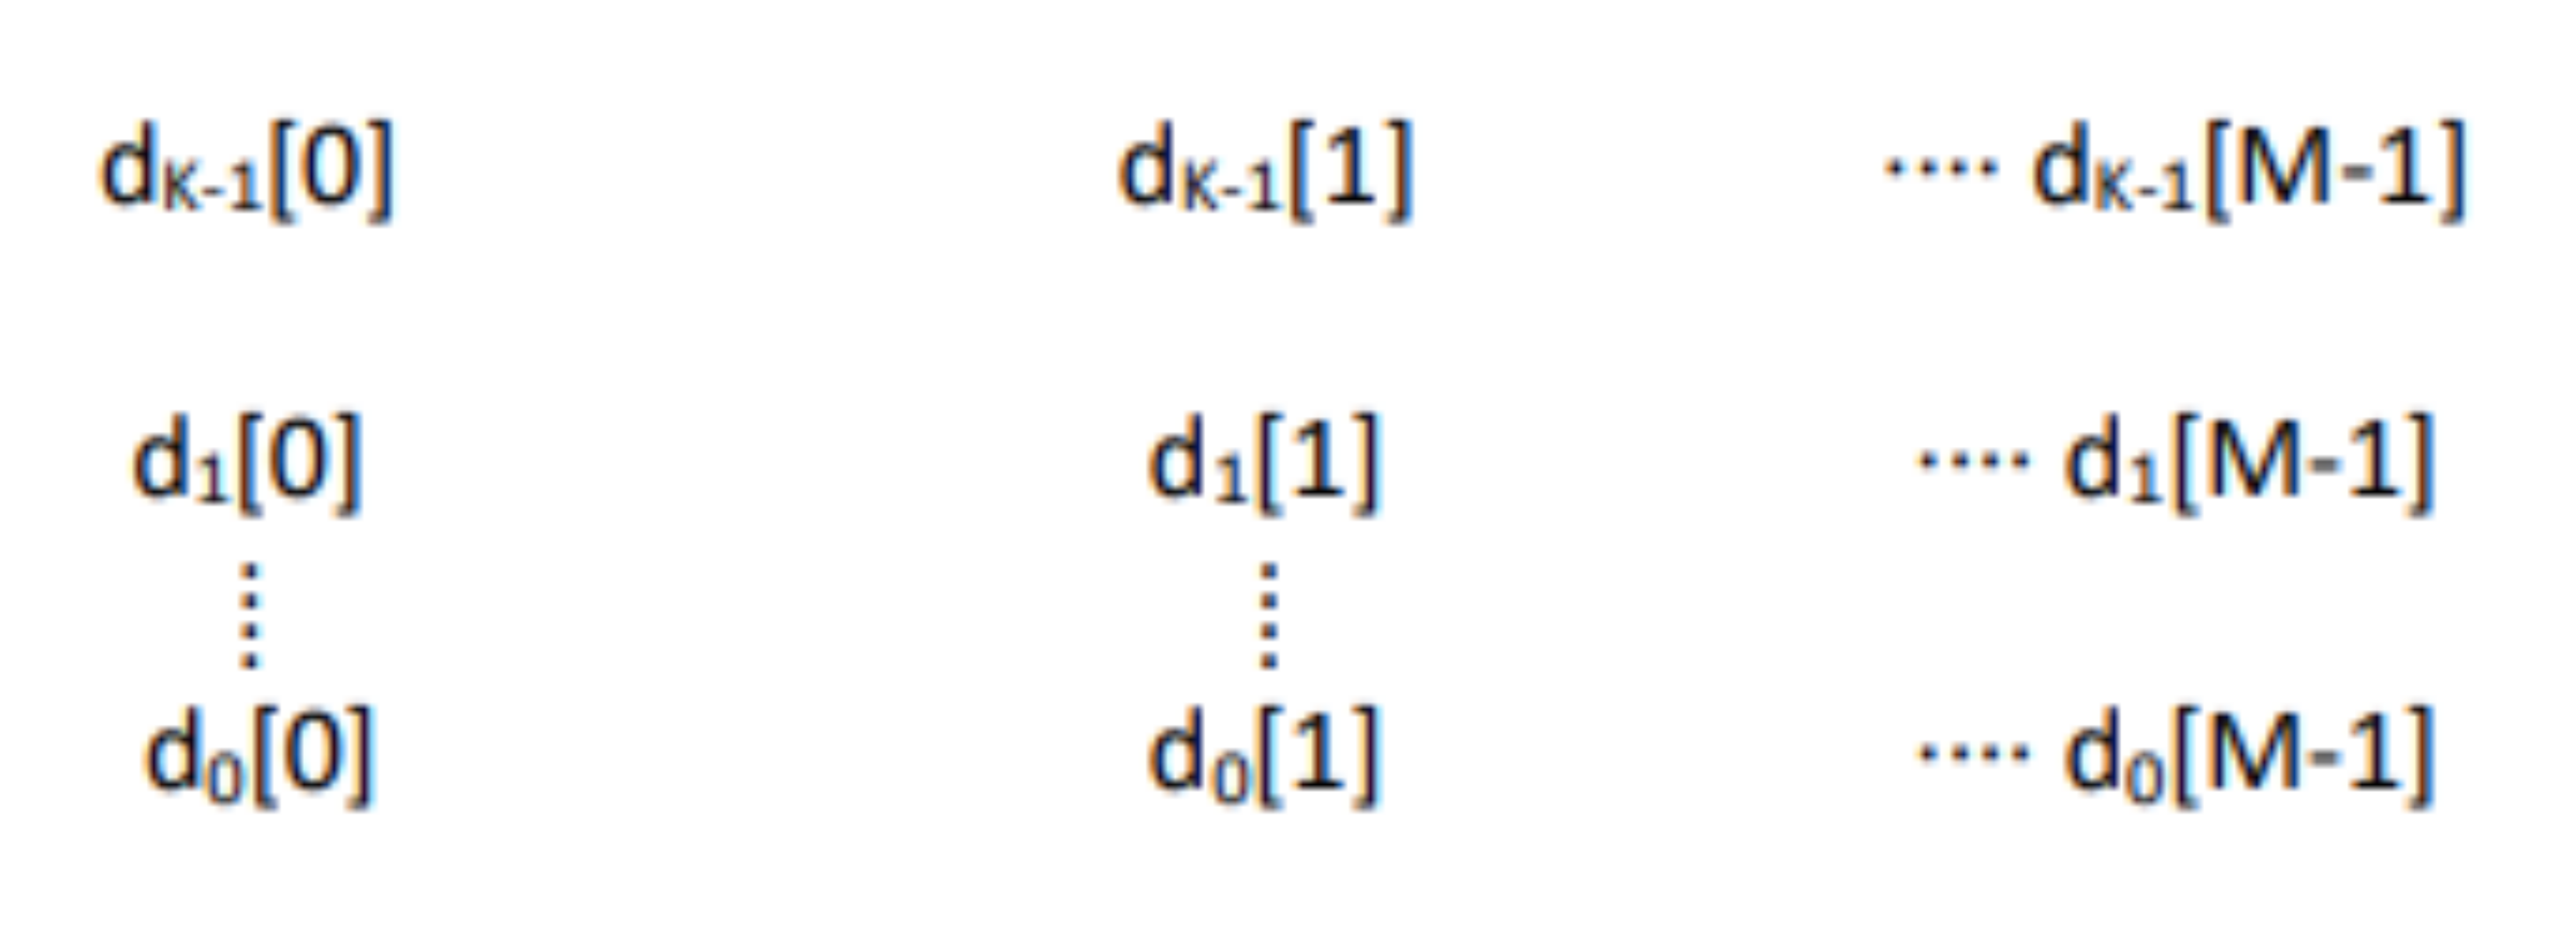
\includegraphics[width=0.6\textwidth]{Imagenes/matriz.png}
%\caption{}
\label{fig:matriz}
\end{figure}

Donde $dk[m]$ representa el símbolo de datos transmitido en la subportadora k-ésima y en el m-ésimo intervalo de tiempo.\\

\begin{figure}[h!]
	\centering
	\includegraphics[width=0.6\textwidth]{Imagenes/DiagBloques.png}
	\caption{Figura1}
	\label{fig:DiagBloques}
\end{figure}
 
En la Figura \ref{fig:DiagBloques} se representa la estructura del transmisor GFDM.\\



En $GFDM$, se pierde la ortogonalidad entre las subportadoras debido al uso de los filtros. Esto ocurre porque los espectros de cada subportadora no se generan a partir de una $FFT$, sino que se ven afectados por la función de transferencia del filtro. Por ello aparece una interferencia entre las subportadoras que empeora la tasa de errores $BER$ (Bit Error Rate) en comparación con $OFDM$. La incidencia de esta interferencia depende del tipo de filtro utilizado. En el caso de filtros en coseno alzado (RRC: RootRaised-Cosine), solo afecta a las subportadoras contiguas, como se ve en la Figura \ref{fig:GFDM}.\\

\begin{figure}[h!]
	\centering
	
\includegraphics[width=0.6\textwidth]{Imagenes/GFDM.png}
	\caption{Portadoras GFDM}
	\label{fig:GFDM}
\end{figure}


La duración del bloque o “trama” $GFDM$ puede adaptarse a las necesidades del servicio a proporcionar. En algunos casos esta duración debe ser muy corta para cumplir el objetivo de latencia de 5G. Se ha analizado un valor de duración igual a la de un símbolo $LTE$. 
En la Figura \ref{fig:GFDM2} se muestra un ejemplo: un intervalo de $LTE$ con 7 símbolos y en el primero de ellos un bloque $GFDM$ con 7 subsímbolos y un único CP.\\

\begin{figure}[h!]
	\centering
	\includegraphics[width=0.6\textwidth]{Imagenes/GFDM2.png}
	\caption{Intervalo LTE}
	\label{fig:GFDM2}
\end{figure}

 

\subsection{Filter Bank Multicarrier (FBMC)}
 
En esta técnica se aplica también un filtrado a cada subportadora como en $GFDM$. Las diferencias están en el tipo de filtro, la modulación de las subportadoras y la temporización de los símbolos. El filtrado prácticamente anula las componentes fuera de banda de cada subportadora, por lo que se reduce drásticamente la necesidad de bandas de guarda. El espectro queda bien confinado dentro de los límites, por lo cual es posible soportar aplicaciones con diferentes necesidades de anchura de banda que requieren fragmentación de espectro. Ahora bien, al ser este filtrado de banda estrecha, se produce una respuesta impulsiva larga en el tiempo (recuérdese que una respuesta abrupta en un dominio, en este caso de la frecuencia, implica justo lo contrario en el otro, generando una prolongación de la señal en el tiempo), lo cual hace que $FBMC$ no resulte idónea para comunicaciones de tipo ráfagas de datos o que necesiten latencia pequeña.\\

Se define y se configura la función de transferencia $HPF$ del filtro prototipo $(PF)$ para una subportadora de referencia. Las funciones de transferencia de los filtros de las subsiguientes subportadoras, se obtienen de la función $HPF$ mediante desplazamientos de frecuencia, ya que las subportadoras poseen idéntico espectro, solo que desplazado en frecuencia. Por ello puede integrarse el procesado $IFFT$ con la generación de las respuestas impulsivas de los filtros en la llamada red polifase (PPN-FFT, una técnica que permite mantener el tamaño de la FFT, pero añadiendo filtros digitales). Debido a este proceso, tanto en GFDM como en $FBMC$ se habla de subcanales en vez de subportadoras, ya que este último término se reserva para el espectro de las señales generadas exclusivamente mediante $IFFT$, utilizándose en cambio el de canales para aquellas que ya no se ajustan a este proceso, como es el caso de la combinación con un filtrado posterior.\\

Se ha estudiado un filtro prototipo paso bajo que satisface el criterio de Nyquist, el cual se especifica mediante muestras en el dominio de la frecuencia. La respuesta impulsiva tiene una longitud $L = 2K-1$, siendo $K$ un factor de diseño, llamado factor de solapamiento que indica el número de muestras de la función de transferencia.
Además, si $M$ es el número de subcanales, se comprueba que el factor de solapamiento está relacionado con $M$, mediante $K = \frac{L}{M}$ y expresa también el número de símbolos que se solapan en el tiempo.\\

El procesado conjunto requiere una $IFFT$ de tamaño $K*M$. Cuanto más alto es el valor de K, mayor es la atenuación fuera de banda, pero también lo es la complejidad. En los análisis se ha elegido un valor $K=4$ como un buen compromiso entre desempeño y complejidad.\\
 
Con los filtros que se han propuesto, aparece una interferencia entre subportadoras contiguas. La subportadora k-ésima interfiere con las $k-1$ y $k+1$ vecinas, pero no con las demás; es decir, las subportadoras pares o impares no interfieren entre sí. Esta es una diferencia con $OFDM$, donde todas las subportadoras han de ser ortogonales, mientras que en $FBMC$ la ortogonalidad solo se precisa para los canales contiguos.\\
 
Para mantener la ortogonalidad en los dominios del tiempo y de la frecuencia, se usa la modulación $QAM$ desplazada O-QAM (Offset QAM). La parte real de los símbolos de la constelación modula las subportadoras pares en los instantes nT y la parte imaginaria las subportadoras impares en los instantes $nT+\frac{T}{2}$. De este modo, no hay interferencia entre los datos. En consecuencia, para transmitir $N$ símbolos hacen falta $2N$ subportadoras. Debido a esa disposición intercalada de los símbolos, no hay reducción de tasa binaria. El uso de esta técnica de modulación junto con los filtros antes mencionados hace que no sea preciso recurrir a un prefijo cíclico. De ahí que esta solución se base en una convolución lineal y no cíclica.\\
 
En las operaciones de $OFDM$ donde no sea preciso el uso del $CP$ (por ejemplo en la inicialización), la modulación $CP-OFDM$ de $LTE$ es un caso particular de $FBMC$ cuando el filtro prototipo es rectangular y el factor de solapamiento es la unidad. Por ello, como ventajas destacables, $FBMC$ es compatible con sistemas basados en $OFDM$ en aquellas fases donde no se utilice el $CP$, es espectralmente más eficiente al no necesitar un prefijo cíclico, no necesita de la sincronización de los terminales móviles y es aplicable a entornos de uso en bandas no contiguas o radio cognitiva, si bien, como inconvenientes, presenta todavía algunos problemas para su aplicación en entornos $MIMO$ y una alta relación $PAPR$ que debe contrarrestarse con algoritmos eficientes, así como el mencionado de la baja eficiencia espectral cuando se transmiten ráfagas cortas de datos, lo que puede ser el caso de aplicaciones $M2M$ o $IoT$ en 5G.\\


\begin{figure}[h!]
	\centering
	
\includegraphics[width=0.6\textwidth]{Imagenes/FBMC.png}
	\caption{Señales FBMC}
	\label{fig:FBMC}
\end{figure}

En la Figura \ref{fig:FBMC}, se representan espectros obtenidos por simulación de señales $FBMC$ con diferentes valores del factor de solapamiento en comparación con $OFDM$. Puede observarse la gran atenuación de los componentes fuera de banda de las señales $FBMC$.\\ 

\subsection{Universal Filtered Multicarrier (UFMC)}

Se ha visto que en $FBMC$ debido al filtrado individual, la respuesta impulsiva es larga. Puede pensarse en hacer un filtrado global de todas las subportadoras. Esta técnica se llama $OFDM$ filtrada (F-OFDM) y con ella la respuesta impulsiva es más corta, pero se pierde flexibilidad en la configuración del espectro.\\

Una solución de compromiso es hacer un filtrado no en una ni en todas, sino en grupos de subportadoras. Para ello se divide el espectro en B sub-bandas, con kb subportadoras en la sub-banda b.
Como casos particulares, $UFMC$ coincide con $FBMC$ para $B=1$ y con $F-OFDM$ para $kb= K$ 
$UFMC$ por su mejor respuesta impulsiva resulta idónea para aplicaciones que implican transmisión de datos en forma de ráfagas cortas y con baja latencia. Tampoco requiere $CP$, y por tanto utiliza convolución lineal. Sin embargo, requiere de una $FFT$ de mayor tamaño, lo que puede complicar los receptores. Asimismo, dado que se pierde parte de la ortogonalidad compleja, podría plantear problemas en aplicaciones de alta tasa de bits. \\

La elección de B depende del escenario de aplicación y el tipo de espectro. Si se trata de un escenario con espectro fragmentado, B elegirá de conformidad con el número de sub-bandas disponibles, pudiendo incluso variar con el tiempo. Puede elegirse B igual a un bloque de recursos RB o a un número entero de RBs de LTE, lo cual facilita la compatibilidad con LTE. También es posible seleccionar el tipo y características de los filtros. Se han ensayado y evaluado filtros FIR con coeficientes definidos por ventanas (Dolph-Chebychev) que son parametrizables en su forma y atenuación de los lóbulos laterales.\\
 

\begin{figure}[h!]
	\centering
	
\includegraphics[width=0.6\textwidth]{Imagenes/UMC.png}
	\caption{Espectros UFMC y OFDM}
	\label{fig:UMC}
\end{figure}

En la figura \ref{fig:UMC}, se muestran espectros de UFMC y OFDM obtenidos por simulación. Se observa la gran atenuación de las componentes fuera de banda de la señal UFMC en comparación con las de la señal OFDM.\\ 

\begin{figure}[h!]
	\centering
	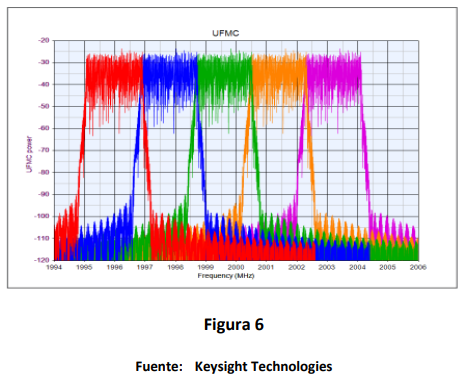
\includegraphics[width=0.6\textwidth]{Imagenes/UMC2.png}
	\caption{Ejemplo multiplexación UMC}
	\label{fig:UMC2}
\end{figure}


Puede aprovecharse esta característica de UFMC para multiplexar en frecuencia sub-bandas con subportadoras correspondientes a diferentes servicios y no necesariamente de la misma anchura, es decir, con espectros fragmentados. 
En la Figura \ref{fig:UMC2} se muestra un ejemplo de multiplexación de 5 sub-bandas. Se aprecia que pueden coexistir con mínima interferencia mutua.\\ 

\subsection{Formas de onda no derivadas de OFDM: Bi-Orthogonal Frequency Division Multiplexing (BFDM) 
	}
	

Además de las soluciones ligadas a mejoras o modificaciones de la modulación $OFDM$, existe un propuesta con un enfoque diferente, que consideramos de interés mencionar aquí: Bi-Orthogonal Frequency Division Multiplexing (BFDM), y que seguidamente se expone. 
En BFDM se aplica un procesado que transforma la ortogonalidad del conjunto de impulsos transmitidos y recibidos en una bi-ortogonalidad, en la cual las representaciones tiempo-frecuencia de esos impulsos son ortogonales por parejas, no individualmente. Esto es, se utilizan impulsos diferentes en emisión y en recepción, en lugar del mismo, como en el caso de OFDM, lo que proporciona mayor flexibilidad en lo relativo a supresión de lóbulos laterales, respuesta impulsiva de los filtros y complejidad de realización práctica. En definitiva, en lugar de basar la cadena de transmisión en un mismo tipo de filtro prototipo para conformar la señal en emisión y recepción, se adopta un enfoque más flexible, donde es posible utilizar diferentes filtros en cada parte, a condición de que ambos impulsos sean ortogonales. Se ha comprobado que gracias a esta flexibilidad puede configurarse la BFDM para que resulte adecuada para tráficos esporádicos como los que en 5G aparecerán, y serán importantes, en comunicaciones entre máquinas MTC (Machine Type Communications).\\

Se ha investigado la integración de $BFDM$ en el estándar $LTE$ para encaminar estos tráficos esporádicos de mensajes cortos y en ráfagas, por el canal físico de acceso aleatorio (PRACH) de $LTE$. Como es sabido, todo el tráfico de datos ascendentes en $LTE$ sea del tipo que sea se transporta por el canal compartido $PUSCH$. La utilización del $PUSCH$ para aquellos tipos de tráfico es muy ineficiente debido a la carga de señalización. Dado que en la configuración del $PRACH$ en $LTE$ hay un intervalo de guarda para separar el $PRACH$ del $PUSCH$, con elementos de recursos no utilizados, estos pueden aprovecharse para cursar este tipo de tráfico.
Por todo ello, se ha propuesto la creación de un nuevo canal en $LTE$ denominado $D-PRACH$ (Data PRACH) para soportar estos tipos de transmisiones asíncronas, con lo que se descargaría el canal $PUSCH$ y se reduciría notablemente la tasa (overhead) de señalización.\\

En el procesado $D-PRACH$, la secuencia de impulsos de los datos produce una conformación del espectro de la señal preámbulo del canal $PRACH$ usando las bandas de guarda de dicho canal con una interferencia aceptable.\\

La biortogonalidad y la longitud relativamente grande de los símbolos de $PRACH$ hacen que $BFD$M sea más robusto que $OFDM$ frente a fluctuaciones de frecuencia y ruido de fase en transmisión. $BFDM$ conserva las ventajas de $CP-OFDM$, en cuanto a interferencia entre símbolos y efecto multitrayecto con el uso de $CP$ y resulta fácil de implementar con el procesado $FFT$.
Sin embargo debe afrontar el efecto de las colas de impulso largas que reducen la eficiencia de la transmisión por ráfagas.\\

\subsection{Nuevos enfoques en las técnicas de acceso: NOMA y SCMA }

Además de las nuevas propuestas en materia de formas de onda, también se están considerando posibles nuevas alternativas para los métodos de acceso múltiple, como son $NOMA$ y $SCMA$, que se describen brevemente a continuación.\\

\subsubsection{Non Orthogonal Multiple Access (NOMA) }

Las anteriores técnicas se basan en el uso de los dominios temporales y de la frecuencia para conseguir repartir el medio de acceso entre varios usuarios. Sin embargo, es posible también utilizar el de la potencia, donde, en lugar de buscar la ortogonalidad para asegurar la ausencia de potencia interferente de otros usuarios, se tolere y se busque esta interferencia para conseguir una mayor eficiencia espectral. Algo que, a primera vista, puede parecer contradictorio. Sin embargo no lo es tanto si se piensa que, en soluciones como en $OFDM$, lo que se hace es asignar una parte del ancho de banda (subportadoras) para un usuario dado en un momento dado. Si en este caso, el canal es de mala calidad, se produce una deficiente eficiencia espectral. En las soluciones no ortogonales, lo que se hace es permitir que todos los usuarios accedan a toda la banda, lo que hace posible que otros usuarios con buena calidad de canal puedan acceder a partes de la banda que antes tendrían vedadas por causa de la parcelación entre usuarios antes mencionada. Y eso resulta en una mayor eficiencia espectral (la suma de las tasas de bit conseguidas con varios usuarios en esa porción de la banda es mayor que si solo la utilizase un solo usuario), aunque el usuario con pobres condiciones de canal experimente algo más de interferencia. Para conseguir dichas mejoras se están estudiando métodos de multiacceso que requieren diseños avanzados de los sistemas receptores para reducir las interferencias inter e intracelulares. Uno de los que han despertado mayor interés es denominado NOMA en el cual la multiplexación clásica de usuarios realizada con recursos ortogonales, se reemplaza por una multiplexación en el dominio de la potencia en el transmisor, conjugada con una separación de usuarios en el receptor, basada en la cancelación sucesiva de interferencia, SIC (Successive Interference Cancellation). En cierto modo, NOMA guarda similitud con el concepto de radio cognitiva, conforme la denominada estrategia “underlay” de funcionamiento. En ella se asume que unos usuarios primarios, que tienen prioridad, utilizan el espectro en convivencia con otros usuarios secundarios, de manera que ello no impide a los usuarios primarios disfrutar de conexiones con una calidad mínima. NOMA se basaría en simultanear las transmisiones de varios usuarios, de forma que exista cierta interferencia entre ellos, asegurando que los más desfavorecidos dispongan de una calidad mínima de recepción, tal y como se hace en la radio cognitiva, pero, a diferencia de esta, en lugar de adaptar la recepción a un entorno que viene impuesto, es el sistema el que define dicho entorno, asignando convenientemente las potencias a cada usuario, de manera que la convivencia en un mismo espectro sea posible y se maximice la tasa global de bits en el espectro utilizado.\\

Este tipo de multiplexación puede aplicarse tanto al enlace ascendente como al descendente. 
En lo que sigue describiremos de forma simplificada en NOMA para el enlace descendente y comprobaremos con un cálculo sencillo la mejora que puede proporcionar en rendimiento espectral en comparación con un sistema clásico ortogonal. 
Para mayor sencillez, supondremos un caso elemental, con una estación base (eNodoB) transmisora y dos terminales receptores $UE1$ y $UE2$. La anchura de banda la normalizamos a 1 Hz. La base transmite al $UE1$ la señal $x1$ con potencia $p1$ y el $UE2$ la señal $x2$ con potencia $p2$. Para cada enlace, la función ganancia del canal radio es hi y el valor de la interferencia intercelular más el ruido térmico es $ni (i=1, 2)$.\\
 
En NOMA de enlace descendente, se realiza la decodificación de las señales en los UE según el orden de valores decrecientes de la relación $|h_i |^2/n_i$ . Según este criterio, se supone que el $UE-i$ puede eliminar la interferencia interusuario del $UE-j$ si $|h_j |^ 2 /n_j < |h_i |^2/n_i$
 
En el caso de 2 usuarios, suponiendo que $|h_1 |^ 2/n_1 > |h_2 |^2/n_2$ , el $UE-2$ decodifica la señal el primero, por lo que no aplica cancelación de interferencia. Por su parte, el $UE-1$ decodifica la señal $x2$ y la resta de la señal recibida $y1$ y a continuación decodifica $x1$ ya sin la interferencia del $UE2$.\\

En el caso ideal de carencia de errores de decodificación, los rendimientos espectrales de cada enlace, serán:\\

\begin{itemize}
	\item Enlace 1: $\eta_1(\frac{b}{s}[Hz])=log_2(1+\frac{p_1|h_1|^ 2}{n_1})$
	\item Enlace 2: $\eta_2(\frac{b}{s}[Hz])=log_2(1+\frac{p_2|h_2|^ 2}{p_1|h_2|^ 2+n_2})$
\end{itemize}

Se desprende de estas expresiones la influencia de la asignación de las potencias $p_1$ y $p_2$ a cada enlace. Al enlace con mayor ganancia de canal se le asigna menor potencia y al que tiene menor ganancia se le asigna mayor ponencia.\\

Por ejemplo, consideremos una situación de bastante disparidad, para la que $|h_1 |^2/n_1$ es $100 (20 dB)$ y $|h_2 |^2/n_2$ es $1 (0dB)$. Aplicando las fórmulas anteriores, para una potencia total normalizada igual a 1 se encuentra:\\

\begin{itemize}
	\item $p_1=0.2,p2=0.8$, $\eta_1=4.39\frac{b}{s}[Hz]$ y $\eta_2=0.74\frac{b}{s}[Hz]$
		\item $p_1=0.5,p2=0.5$, $\eta_1=5.67\frac{b}{s}[Hz]$ y $\eta_2=0.41\frac{b}{s}[Hz]$
\end{itemize} 

Se ve que el reparto desigual de la potencia favorece al usuario con peor relación señal/ruido, a costa de empeorar la eficiencia del usuario mejor. Si se fuerza más el desequilibrio, por ejemplo con $p_1=0.1$ y $p_2=0.9$ resulta $\eta_1=3.46$ y $\eta_2=0.86$. La ganancia que se registra para el $UE2$ no comprensa la pérdida que se observa en el $UE1$.\\
 
La asignación de potencias diferentes facilita la decodificación correcta con gran probabilidad y por lo tanto la cancelación de la interferencia; la señal destinada al $UE2$ llega con gran nivel al UE1 y puede decodificarse y utilizarse para la cancelación. La señal destinada al $UE1$ llega muy débil a $UE2$ y puede interpretarse como ruido de fondo.\\

Pueden compararse estos resultados con los que se obtendrían con un acceso ortogonal $OMA$ (Orthogonal Multiple Access) en el que tanto la banda de frecuencias asignada a cada usuario como la potencia son las mismas. Esto es cada usuario dispondría de la mitad de la banda y de la mitad de la potencia. Se tendría entonces:\\

\begin{equation}
  \eta_1=0.5log_2(1+\frac{0.5|h_1|^ 2}{0.5n_1})
\end{equation}


\begin{equation}
\eta_2=0.5log_2(1+\frac{0.5|h_1|^ 2}{0.5n_1})
\end{equation}

Y por los mismos valores de la relación señal/ruido que antes se obtiene $\eta_1=3,33 (b/s/Hz)$ y $\eta_2=0,5 (b/s/Hz)$.\\
 
Comparando con los resultados anteriores, para la distribución de potencias $0,2/0,8$, hay unas ganancias porcentuales del 32 porciento para el $UE1$ y el 48 porciento para el $UE2$.\\
 
Naturalmente, $NOMA$ requiere una carga adicional de señalización, con su incidencia en la tasa de los canales físicos de datos.\\

En $NOMA$ la información de estado del canal $CSI$, (Channel State Information) se utiliza en el receptor para la demultiplexación de los usuarios y en el transmisor para decidir el emparejamiento de usuarios y asignación de las potencias.\\

Se están estudiando aspectos prácticos de esta tecnología como son la asignación de potencias, tasa de señalización, propagación de los errores de cancelación de interferencia (SIC), desempeño (performance) en escenarios de alta movilidad, compatibilidad con $MIMO$ e incidencia de la programación (scheduling) de usuarios. Se han obtenido en simulaciones valores de mejora del caudal en $NOMA$ respecto de la técnica ortogonal $OMA$ del orden del 30 porciento para diversas variantes de asignaciones de potencia y programaciones.\\
 
En lo relativo a la incidencia de la propagación de los errores de la $SIC$, no parece que sea muy significativa. Asimismo, los análisis realizados para valorar la influencia de la velocidad de desplazamiento del terminal de usuario, muestran que las ganancias de $NOMA$ sobre $OMA$ se mantienen en torno al 24 porciento para una grama de velocidades de 20 a 100 $[\frac{km}{h}]$.\\
 
El $3GPP$ abrió en 2014 un punto de estudio denominado $MUST$ (downlink MultiUser Superposition Transmission) que incluye técnicas $NOMA$.\\

Sparse Code Multiple Access (SCMA)

En esta tecnología de acceso múltiple con códigos dispersos, con los bits procedentes del codificador de canal (FEC) del transmisor, se efectúa un procesado conjunto de expansión-modulación que transforma bloques de aquellos bits en palabras-código (codewords) extraídas de un repertorio de códigos libro-código (codebook), cuyos elementos son símbolos de una constelación multidimensional.\\

\begin{figure}[h!]
	\centering
	
\includegraphics[width=0.6\textwidth]{Imagenes/SCMA.png}
	\caption{Señal SCMA}
	\label{fig:SCMA}
\end{figure}

En la Figura \ref{fig:SCMA}, se representa el diagrama de bloques. Como se ve la señal SCMA a la salida del procesador se lleva un modulador OFDM convencional.\\

La expansión, aunque similar en concepto a la que se realiza en $CDMA$, difiere de ella en la constitución de los códigos empleados. En $CDMA$, los códigos son “compactos” o densos con todos sus elementos no nulos. $(Valores \pm 1)$.\\
 
En $SCMA$, sin embargo, las palabras-código contienen un gran número de ceros. Por ello se habla de códigos de baja densidad y de expansión dispersa (sparse spreading). Además, estos códigos dispersos están contenidos, como se ha dicho, en un repertorio de códigos diseñados convenientemente, cada uno de los cuales define una capa (layer) y contiene $K=2m$ símbolos, siendo m el número de bits del bloque entrante al módulo expansor. De estos $K$ símbolos $N$ son no nulos y se toman de una constelación multidimensional. La elección de este tipo de constelación se debe a que ofrece mayores posibilidades de distancia mínima entre los puntos de la constelación, lo cual implica en una reducción de la probabilidad de error.\\

Los elementos no nulos ocupan una posición única y exclusiva en cada capa que se denomina patrón de dispersión (sparsity pattern).\\

El número $J$ de capas es igual al de combinaciones de $K$ elementos tomados de $N$ en $N$. Se denomina factor de sobrecarga (overlaid factor) al cociente J/K expresado como porcentaje.\\



\begin{figure}[h!]
	\centering
	
\includegraphics[width=0.6\textwidth]{Imagenes/SCMA8.png}
	\caption{codebook-bit-to-codeword-mapping}
	\label{fig:SCMA8}
\end{figure}



A título de ejemplo, se muestra en la Figura \ref{fg:SCMA8} el esquema de principio de un codificador $SCMA$ con $J = 6$ capas (6 repertorios), para bloques de bits de entrada al tamaño $m = 3$, por lo que cada repertorio contiene $K = 23 = 8$ palabras-código complejas. El tamaño de cada palabra, es decir, la longitud de la expansión es $K = 4$ y el número de elementos no nulos es $N = 2$, por lo que pueden formarse 6 capas. 
Cada bloque de 3 bits de entrada se pone en correspondencia con una palabra-código. En el ejemplo de la figura se muestran, en diferentes colores, las palabras-código asignadas por las capas a los bloques: 011 del usuario 1 (capa 1), 000 del usuario 2,……. y así sucesivamente hasta el bloque 111 del usuario 6.\\


\begin{figure}[h!]
	\centering
	
\includegraphics[width=0.6\textwidth]{Imagenes/OFDM.png}
	%\caption{Figura9}
	\label{fig:OFDM}
\end{figure}


Las palabras código extraídas de cada capa, se suman elemento a elemento y el resultado se aplica, en este ejemplo, a 4 subportadoras OFDM. El conjunto de las subportadoras y palabra-código constituye el llamado Boque SCMA (SCMA block).
En la Figura \ref{fig:OFDM}, se representa, para este mismo ejemplo, el multiacceso de 6 usuarios (uno por cada capa), con sus palabras-código y la formación del bloque $SCMA$.\\

Se observa una característica de este tipo de acceso múltiple que es la superposición de varios elementos de las palabras-código de diferentes usuarios en cada elemento de recursos RE (resource element). Como se ve en el ejemplo el RE1 se solapan símbolos de los usuarios 1, 3 y 5.\\

También puede apreciarse como la expansión de baja densidad reduce el número de colisiones gracias a la existencia de símbolos nulos. En el ejemplo, hay 3 colisiones en vez de las 6 posibles y el factor de sobrecarga es 6/4, es decir el 150 porciento.\\

Un aspecto clave de $SCMA$ es la elección de los repertorios de códigos. Esta se basa en la optimización conjunta del patrón de ensanchamiento disperso (sparse spreading pattern) y la configuración de la modulación multidimensional. El objetivo de diseño es conseguir buenas propiedades de distancia euclídea entre los puntos de las constelaciones para optimizar la ganancia del codificador.\\

La característica de baja dispersión permite utilizar algoritmos de detección/decodificación conjunta de las capas superpuestas. Tales algoritmos son de tipo transferencia de mensajes MPA (Message Passing Algorithms), cuyo desempeño es bastante similar a los algoritmos de máxima verosimilitud ML (máximum Likelihood) clásicos de las comunicaciones digitales. También se aduce que SCMA/MPA puede implementarse con procesadores de transmisión/recepción de complejidad asequible a la tecnología actual.\\
 
$SCMA$, como sistema de multiacceso no ortogonal $NOMA$ que es, puede combinarse con la $NOMA$ de gestión de la potencia para constituir un $NOMA$ híbrido código-potencia, eficaz para el multiacceso de usuarios en escenarios multicelulares.\\

Dentro del grupo $R_1$ del $3gpp$ se ha propuesto un punto de estudio con el fin de investigar más a fondo las aptitudes y posibilidades de $SCMA$ para los escenarios de uso de $5G$, banda ancha móvil ampliada $eMBB$ , comunicaciones masivas de sensores $mMTC$ y comunicaciones muy fiables de baja latencia $URLLC$.\\
 
Comparación de prestaciones 
A modo de resumen final, en la figura \ref{fig:tabla} adjunto se resumen las prestaciones de los distintos métodos con respecto a las características más relevantes.\\

\begin{figure}[h!]
	\centering
	\includegraphics[width=0.6\textwidth]{Imagenes/tabla.png}
	\caption{Comparación de prestaciones}
	\label{fig:tabla}
\end{figure}



\section{¿que tecnicas de acceso se emplearan en 5G?}

\subsection{COMPONENTES}

Al hablar de tecnologías 5G nos referimos a una red de telefonía móvil universal súper
eficiente atenta a la demanda, y donde los recursos son optimizados continuamente para
ofrecer un rendimiento suficiente, con el fin de que los usuarios perciban una conexión a
una red con infinito ancho de banda. Además, el rendimiento de velocidad de datos se ha
optimizado por medio de los diversos componentes presentes en la nueva evolución, que
manejan una baja latencia necesaria para que las aplicaciones que interactúan, se
conviertan en una unificación de términos, el cual hace referencia a la nomenclatura
llamada internet de las cosas.\\
32Revista Electrónica de
Estudios Telemáticos
Esta tecnología es una revolución en la eficiencia, entregando más y mejores redes
para un mejor rendimiento a un menor costo de inversión. La importancia de los diversos
componentes presentes dentro de la llamada revolución de la conectividad de muchos a
muchos, es la esencia central para que toda esta arquitectura de soluciones pueda
funcionar y ofrecer lo que promete ser, destacando los siguientes componentes:

\subsection{TRANSMISIÓN DE MULTI-ANTENNA}
La transmisión de múltiples antenas ya desempeña un papel importante para las
generaciones actuales de comunicaciones móviles y jugará un rol aún más importante en
la era 5G. Especialmente para operar a frecuencias más altas, el uso de múltiples antenas
para formación de haz en el transmisor y/o sitio receptor es un componente crítico para
contrarrestar las peores condiciones de propagación a frecuencias más altas. \\

Sin
embargo, la formación de haz también será un componente importante para frecuencias
más bajas; por ejemplo, para extender aún más la cobertura y proporcionar las tasas de
datos más altas en las implementaciones de esta tecnología. En otras palabras, la
trasmisión de múltiples antenas o nodos, servirán como base sólida con el objetivo de
aumentar el volumen de los datos 1000 veces en comparación a los actuales, así como el
número de dispositivos conectados en las redes.\\

\subsection{DISEÑO ULTRA DELGADO}
El diseño de acceso por radio Ultra-delgado es importante para lograr una alta
eficiencia en las futuras redes de acceso inalámbrico, donde el principio básico se puede
expresar como: minimizar cualquier transmisión que no esté directamente relacionada con
33Revista Electrónica de
Estudios Telemáticos
la entrega de datos del usuario.\\

 El diseño ultra-delgado es especialmente importante para
los despliegues densos con un gran número de nodos en la red y condiciones de tráfico
muy variables; beneficiosas para todo tipo de implementaciones.
Al permitir que los nodos de la red entren rápidamente en estados de baja energía
cuando no hay transmisión de datos de usuario, el diseño ultra-delgado es un
componente importante para el rendimiento de alta energía a la red, de igual manera
permitirá velocidades de datos más altas alcanzables mediante la reducción de la
interferencia de las transmisiones no relacionadas con los datos de usuario.\\

\subsection{SEPARACIÓN DE ACCESO Y CONTROL}
Otro principio de diseño importante para el futuro de acceso inalámbrico es desacoplar
los datos del usuario y el sistema funcional de control. Este último, incluye la información,
así como los procedimientos necesarios para que un dispositivo pueda acceder al
sistema. Un desacoplamiento permitirá una mejor escalabilidad, por ejemplo, los datos de
usuario pueden ser entregados por una densa capa de nodos de acceso, mientras la
información del sistema solo se proporciona a través de una macro capa superpuesta, en
la que inicialmente un dispositivo accede al sistema. Un diseño ultra-delgado combinado
con la separación de acceso y control proporciona una mayor flexibilidad en términos de
evolución de la RAT (Tecnología de Radio Acceso), ya que con esta separación, el plano
de usuario puede evolucionar mientras se mantiene el control funcional del sistema.\\

\subsection{USO DEL ESPECTRO FLEXIBLE}
Desde su creación, la comunicación móvil ha dependido del espectro con licencia en
función de cada operador dentro de un área geográfica. Esto seguirá siendo la base para
la comunicación móvil en la era 5G, permitiendo a los operadores proporcionar
conectividad de alta calidad en un entorno sin interferencias controlada. Sin embargo, la
concesión de licencias por operador del espectro se complementará con la posibilidad de
operar bajo otros regímenes de espectro.
Esto puede incluir el intercambio de espectro entre un conjunto limitado de
operadores, así como la operación en el espectro sin licencia. En las bandas de alta
frecuencia, la atención se centrará en los anchos de banda de transmisión muy amplios,
que normalmente se utilizarán para implementaciones muy densas lo que puede dar
variaciones de tráfico mucho más dinámicas. Estáticamente, dividir el espectro entre
diferentes operadores puede, en tales situaciones, no necesariamente conducir a la
utilización del espectro más eficiente. Más bien, haciendo posible que los operadores
puedan acceder conjuntamente al menos parte del espectro de una manera dinámica lo
que podría conducir a la utilización del espectro global más eficiente.\\

\subsection{FLEXIBLE DUPLEX}
La División de Frecuencia Dúplex (FDD) ha sido dominante desde el comienzo de la
era de la comunicación móvil. Para las bandas de frecuencias más bajas, la FDD seguirá
siendo el principal plan de dúplex en la era 5G. Sin embargo, para las bandas de
34Revista Electrónica de
Estudios Telemáticos
frecuencias más altas, especialmente por encima de 10 GHz, estarán dirigidas en los
despliegues para redes densas. Además, para las variaciones dinámicas de tráfico en
zonas muy densas, la capacidad para asignar dinámicamente recursos de transmisión a
distintas direcciones permitirá una utilización más eficiente del espectro disponible.\\

\subsection{COMUNICACIÓN DIRECTA DISPOSITIVO-A-DISPOSITIVO
	}
	
	La posibilidad de que (D2D) la limitada comunicación directa de dispositivo a
dispositivo ha sido recientemente introducida como una extensión de las especificaciones
de LTE. En la era 5G, el apoyo a D2D como parte de la solución global de acceso
inalámbrico debe ser considerado desde el principio.\\

Esto incluye la comunicación de
datos de usuario punto a punto directamente entre los dispositivos, por ejemplo, el uso de
dispositivos móviles como relés para extender la cobertura de red. Comunicación D2D en
el contexto de 5G debe ser una parte integral de la solución global de acceso inalámbrico
en lugar de una solución independiente.
La posibilidad de comunicación directa debería ampliar las capacidades y mejorar la
eficiencia global de la red de acceso inalámbrico. Además, con el fin de evitar la
interferencia incontrolada a otros enlaces, la comunicación D2D debe estar bajo control de
la red, especialmente importante para el caso de D2D con espectro licenciado.\\

\subsection{INTEGRACION ACCESO/BACKHAUL}

El Backhaul corresponde a la porción de una red jerárquica, que comprende los
enlaces intermedios entre el núcleo o backbone, y las subredes en sus bordes. En este
sentido, la tecnología inalámbrica se utiliza con frecuencia como parte de la solución de
Backhaul, donde tales soluciones operan bajo la línea de visibilidad directa bajo las
condiciones que utilizan la tecnología de radio de propiedad en las bandas de frecuencias
más altas, incluyendo la banda de ondas milimétricas (MMW).\\

En el futuro, el enlace de acceso (estación base a dispositivo) también se extenderá a
frecuencias más altas. Además, para apoyar las implementaciones de baja potencia, los
Backhaul inalámbricos tendrán que extenderse a cubrir espacios sin línea de visión, en
condiciones similares a los enlaces de acceso. Según Ericsson (2014) en la era 5G, el
enlace de acceso inalámbrico y Backhaul inalámbrico por lo tanto no deben ser vistos
como dos entidades separadas con soluciones técnicas independientes. Más bien,
Backhaul y acceso deben ser vistos como una solución de acceso inalámbrico integrado
capaz de utilizar la misma tecnología básica y operar bajo un espectro en común. Esto
dará lugar a una utilización más eficiente del espectro global, así como la operación
reducida y el esfuerzo de gestión

\section{ ¿Cuáles son las bandas RF para 5G?}






\subsection{Generacion 5G}


Cada generación nueva de red inalámbrica trajo aparejados nuevos conjuntos de casos de uso. La tecnología 5G no va a ser
la excepción y va a centrarse en el IoT y en las aplicaciones de comunicaciones críticas.\\

Las redes 5G expanden los servicios inalámbricos de banda ancha más allá del Internet móvil al IoT y a
segmentos de comunicaciones críticas Las redes 4.5G (LTE advanced) duplican la velocidad de los datos de la
tecnología 4G.\\


La implementación de las redes 5G, a la vez que se mantienen
operativas las redes 3G y 4G, probablemente den lugar a un nuevo
desafío para los operadores de redes móviles con respecto a la
capacidad de las frecuencias en el espectro (sobre todo si se
produce el enorme volumen previsto en el IoT). Los operadores de
redes.\\




\begin{figure}[h!]
	\centering
	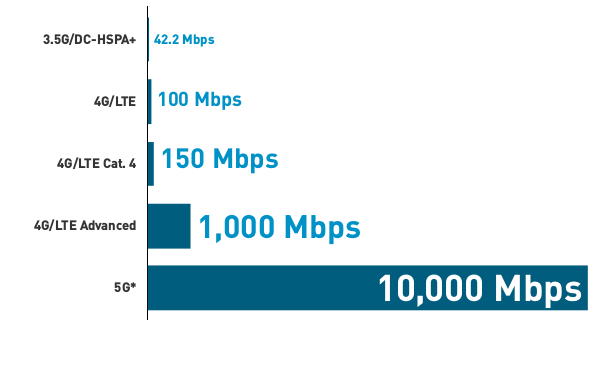
\includegraphics[width=0.6\textwidth]{Imagenes/sist3.png}
	\caption{Tasa de transferencia de datos entre generaciones}
	\label{fig:sist3}
\end{figure}

\section{Referencias}


Conor Sexton et al. “5G: Adaptable Networks Enabled by Versatile Radio Access
Technologies”. IEEE COMMUNICATIONS SURVEYS and TUTORIALS, VOL. 19, NO. 2,\\

SECOND QUARTER 2017
16 de 192. S.M. Riazul Islam et al. “ Power-Domain Non-Orthogonal Multiple Access (NOMA) in
5G Systems: Potentials and Challenges “. IEEE COMMUNICATIONS SURVEYS and
TUTORIALS, VOL. 19, NO. 2, SECOND QUARTER 2017\\

3. Behrouz Farhang-Boroujeny et al. “OFDM Inspired Waveforms for 5G”. IEEE
COMMUNICATIONS SURVEYS and TUTORIALS, VOL. 18, NO. 4, FOURTH QUARTER 2016.\\

4. Mamta Agiwal et al. “Next Generation 5G Wireless Networks: A Comprehensive
Survey”. IEEE COMMUNICATIONS SURVEYS and TUTORIALS, VOL. 18, NO. 3, THIRD
QUARTER 2016\\

5. DING, Zhiguo, et al. “Application of non-orthogonal multiple access in LTE and 5G
networks”. IEEE Communications Magazine, 2017, vol. 55, no 2, p. 185-191.\\

6. SCHAFHUBER, “Dieter et al. Pulse-shaping OFDM/BFDM systems for time-varying
channels: ISI/ICI analysis, optimal pulse design, and efficient implementation”.
Personal, Indoor and Mobile Radio Communications, 2002. The 13th IEEE International
Symposium on. IEEE, 2002. p. 1012-1016.\\

7. WUNDER, Gerhard, et al. “5GNOW: non-orthogonal, asynchronous waveforms for
future mobile applications”. IEEE Communications Magazine, 2014, vol. 52, no 2, p. 97-
105.\\



%\bibliographystyle{plain}
%\bibliography{Referencias.bib}



\end{document}
